\begin{frame}{}
	\centering \textbf{\huge General graphs}
\end{frame}

\begin{frame}[t]{General graphs}
	\textbf{Problem:} odd-length cycles\\
	%images with 6 edges, 5 edges in a cycle and one more adjacent edge
	
	\begin{center}
	Maximal: matching of size 2
	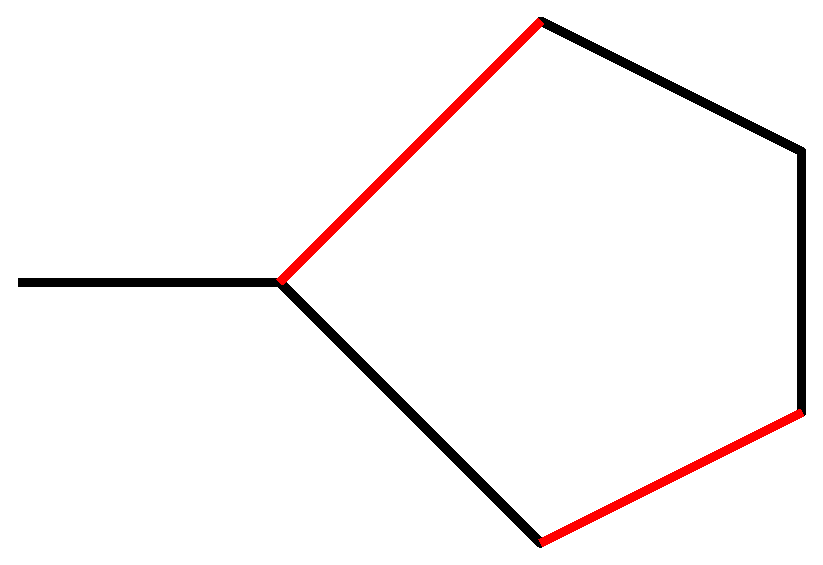
\includegraphics[width=0.35\linewidth]{img/general/odd-matching-maximal.eps}
	\end{center}

	\begin{center}
	Optimum: matching of size 3
	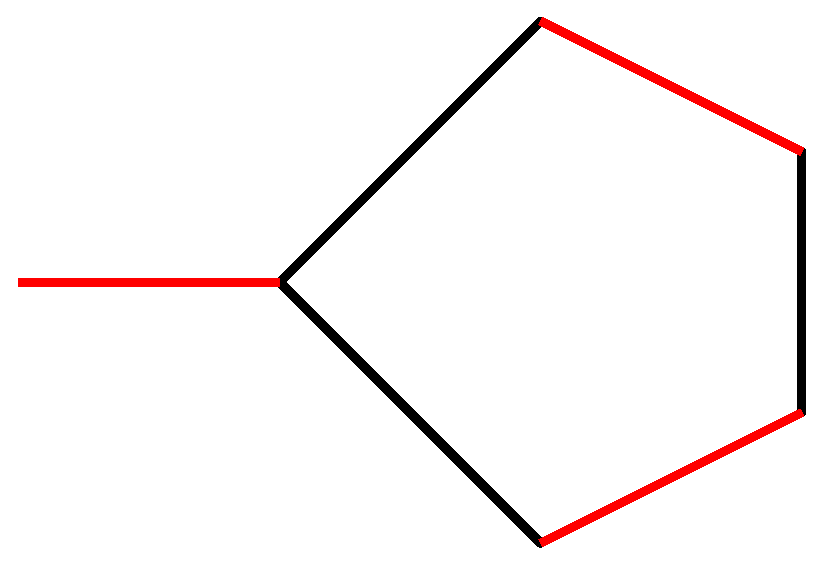
\includegraphics[width=0.35\linewidth]{img/general/odd-matching-optimal.eps}
	\end{center}
\end{frame}

\begin{frame}[t]{General graphs}
	Bipartite graphs can have cycles, but always only of even length:\\
	
	\begin{center}
	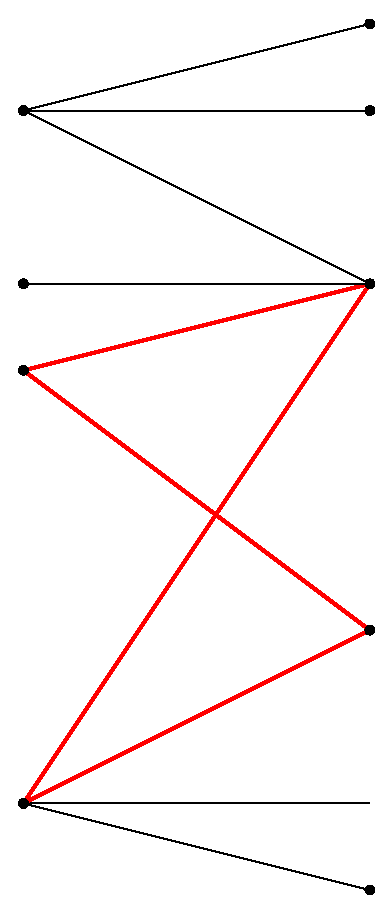
\includegraphics[width=0.2\linewidth]{img/general/bipartite-even-cycle.eps}	
	\end{center}	
\end{frame}

\begin{frame}[t]{Edmonds' Blossom algorithm (1961)}
	\only<1->{Blossom algorithm uses the idea of Berge's Theorem, that}
	
	\only<2->{matching is a \textbf{maximum matching} iff there is \textbf{no augmenting path}.}
	
	\only<3->{
		\vspace{1em}
		\textbf{Input:} Graph $\mathcal{G}$, initial matching $\mathcal{M}$ on $\mathcal{G}$\\
		\textbf{Output:} maximum matching $\mathcal{M^*}$ on $\mathcal{G}$	
	}

	\only<4->{
		\vspace{1em}
		In other words, Blossom algorithm improves existing matching $\mathcal{M}$ in $\mathcal{G}$ as long as augmenting paths exist, then returns.	
	}
\end{frame}

\begin{frame}[t]{Edmonds' Blossom algorithm (1961)}
	\begin{center}
	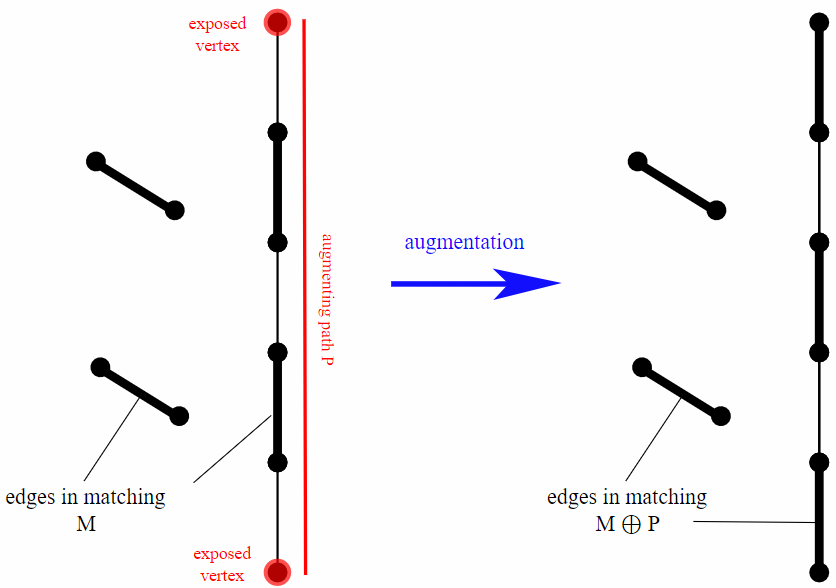
\includegraphics[width=0.8\linewidth]{img/general/Edmonds_augmenting_path.png}
	\end{center}
\end{frame}

\begin{frame}[t]{Edmonds' Blossom algorithm (1961)}
	\only<1->{
		\textbf{Problem:} How to guarantee no augmenting paths in a graph?
	}

	\only<2->{
		\vspace{1em}
		\textbf{Schema:} 
		\begin{itemize}
			\item shrink the graph in a way, that preserves augmenting paths
			\item extend matching when possible
			\item return, when no augmenting path found
		\end{itemize}
	}
\end{frame}

\begin{frame}[t]{Edmonds' Blossom algorithm (1961)}
	\textbf{Example:}
	
	[TODO: include images]
\end{frame}

\begin{frame}[t]{Edmonds' Blossom algorithm (1961)}
	\textbf{Pseudocode:}\\
	[TODO: include pseudocode]
	
	\vspace{1em}
	\textbf{Complexity:} [TODO: include complexity]

\end{frame}